\documentclass{beamer}

% Theme choice
\usetheme{Madrid}

% Packages
\usepackage{amsmath, amssymb, amsfonts}
\usepackage{graphicx}
\usepackage{hyperref}
\usepackage{xcolor}
\usepackage{tikz}

% Title and author information
\title{NCERT 9.1.4: Solving a Nonlinear ODE}
\author{Krishna Patil - EE24BTECH11036}
\date{\today}

\begin{document}

% Title slide
\begin{frame}
    \titlepage
\end{frame}

% Outline slide
\begin{frame}{Outline}
    \tableofcontents
\end{frame}

% Problem statement
\section{Problem Statement}
\begin{frame}{Problem Statement}
    Solve the following nonlinear ODE:
    \begin{equation*}
        \left(\frac{d^2y}{dx^2}\right)^2 + \cos\left(\frac{dy}{dx}\right) = 0.
    \end{equation*}
\end{frame}

% Reformulating the equation
\section{Reformulating the Equation}
\begin{frame}{Reformulating the Equation}
    Define:
    \begin{align*}
        v &= \frac{dy}{dx}, \\
        u &= \frac{d^2y}{dx^2}.
    \end{align*}
    Substituting into the equation gives:
    \begin{equation*}
        u^2 + \cos(v) = 0.
    \end{equation*}
    \vspace{0.5cm}
    Solve for $u$:
    \begin{equation*}
        u = \pm \sqrt{-\cos(v)}, \quad \text{valid only for } \cos(v) < 0.
    \end{equation*}
\end{frame}

% Numerical Method: RK4
\section{Numerical Method: RK4}
\begin{frame}{Numerical Method: RK4}
    \textbf{System of Equations:}
    \begin{align*}
        \frac{dy}{dx} &= v, \\
        \frac{dv}{dx} &= \pm \sqrt{-\cos(v)}.
    \end{align*}
    \vspace{0.5cm}
    \textbf{RK4 Updates for $y$:}
    \begin{align*}
        k_{y,1} &= h \cdot v, \\
        k_{y,2} &= h \cdot \left(v + \frac{k_{v,1}}{2}\right), \\
        k_{y,3} &= h \cdot \left(v + \frac{k_{v,2}}{2}\right), \\
        k_{y,4} &= h \cdot \left(v + k_{v,3}\right), \\
        y_{n+1} &= y_n + \frac{1}{6}\left(k_{y,1} + 2k_{y,2} + 2k_{y,3} + k_{y,4}\right).
    \end{align*}
\end{frame}

\begin{frame}{Numerical Method: RK4 (contd.)}
    \textbf{RK4 Updates for $v$:}
    \begin{align*}
        k_{v,1} &= h \cdot \sqrt{-\cos(v)}, \\
        k_{v,2} &= h \cdot \sqrt{-\cos\left(v + \frac{k_{v,1}}{2}\right)}, \\
        k_{v,3} &= h \cdot \sqrt{-\cos\left(v + \frac{k_{v,2}}{2}\right)}, \\
        k_{v,4} &= h \cdot \sqrt{-\cos\left(v + k_{v,3}\right)}, \\
        v_{n+1} &= v_n + \frac{1}{6}\left(k_{v,1} + 2k_{v,2} + 2k_{v,3} + k_{v,4}\right).
    \end{align*}
\end{frame}

% Implementation Steps
\section{Implementation Steps}
\begin{frame}{Implementation Steps}
    \begin{enumerate}
        \item Choose initial values $y(0) = y_0$ and $v(0) = v_0$.
        \item Select a step size $h$ to control accuracy.
        \item Alternate updates for $y$ and $v$ using RK4 equations.
        \item Ensure $\cos(v) < 0$ during integration for validity.
    \end{enumerate}
\end{frame}

% Results and Visualization
\section{Results and Visualization}
\begin{frame}{Results and Visualization}
    Below is the plot of $y$ vs $x$ obtained using the RK4 method:
    \begin{figure}[h]
        \centering
        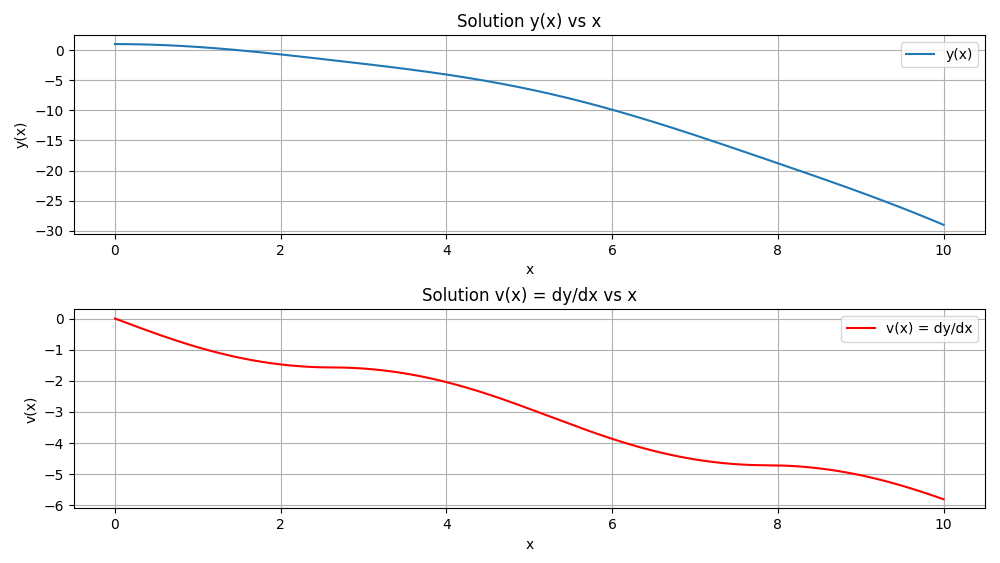
\includegraphics[width=0.8\textwidth]{fig/Figure_1.png}
        \caption{Numerical Solution of the ODE}
        \label{fig:example}
    \end{figure}
\end{frame}

% Conclusion
\section{Conclusion}
\begin{frame}{Conclusion}
    \begin{itemize}
        \item Solved the nonlinear ODE using the RK4 method.
        \item Demonstrated the solution's dependence on initial conditions and step size.
        \item Plots confirm the validity of the numerical solution.
    \end{itemize}
\end{frame}

\end{document}

